\documentclass[border=0pt]{standalone}
\usepackage{graphicx}
\usepackage{tikz}
\usepackage{helvet}
\renewcommand{\familydefault}{\sfdefault}
\usetikzlibrary{calc}
\definecolor{ba}{HTML}{505ED5}
\definecolor{argos}{HTML}{D74D3D}
\definecolor{sindy}{HTML}{8EB63D}
\newcommand{\Tag}[1]{{\fontsize{8}{9}\selectfont\bfseries #1}}
\newcommand{\Lab}[1]{{\fontsize{7}{8}\selectfont #1}}
\begin{document}
\begin{tikzpicture}[x=1mm,y=-1mm]
\node[anchor=north, inner sep=0pt] at (43.000,0.000) {\Lab{Against \textit{n} at SNR = 49 dB}};
\node[anchor=north, inner sep=0pt] at (123.000,0.000) {\Lab{Against SNR at \textit{n} = 5000}};
\node[anchor=center, inner sep=0pt, rotate=90] at (2.000,42.500) {\Lab{Bayesian-ARGOS}};
\node[anchor=north west, inner sep=0pt] at (3.500,4.000) {\Tag{a}};
\node[anchor=north west, inner sep=0pt] at (5.000,4.500) {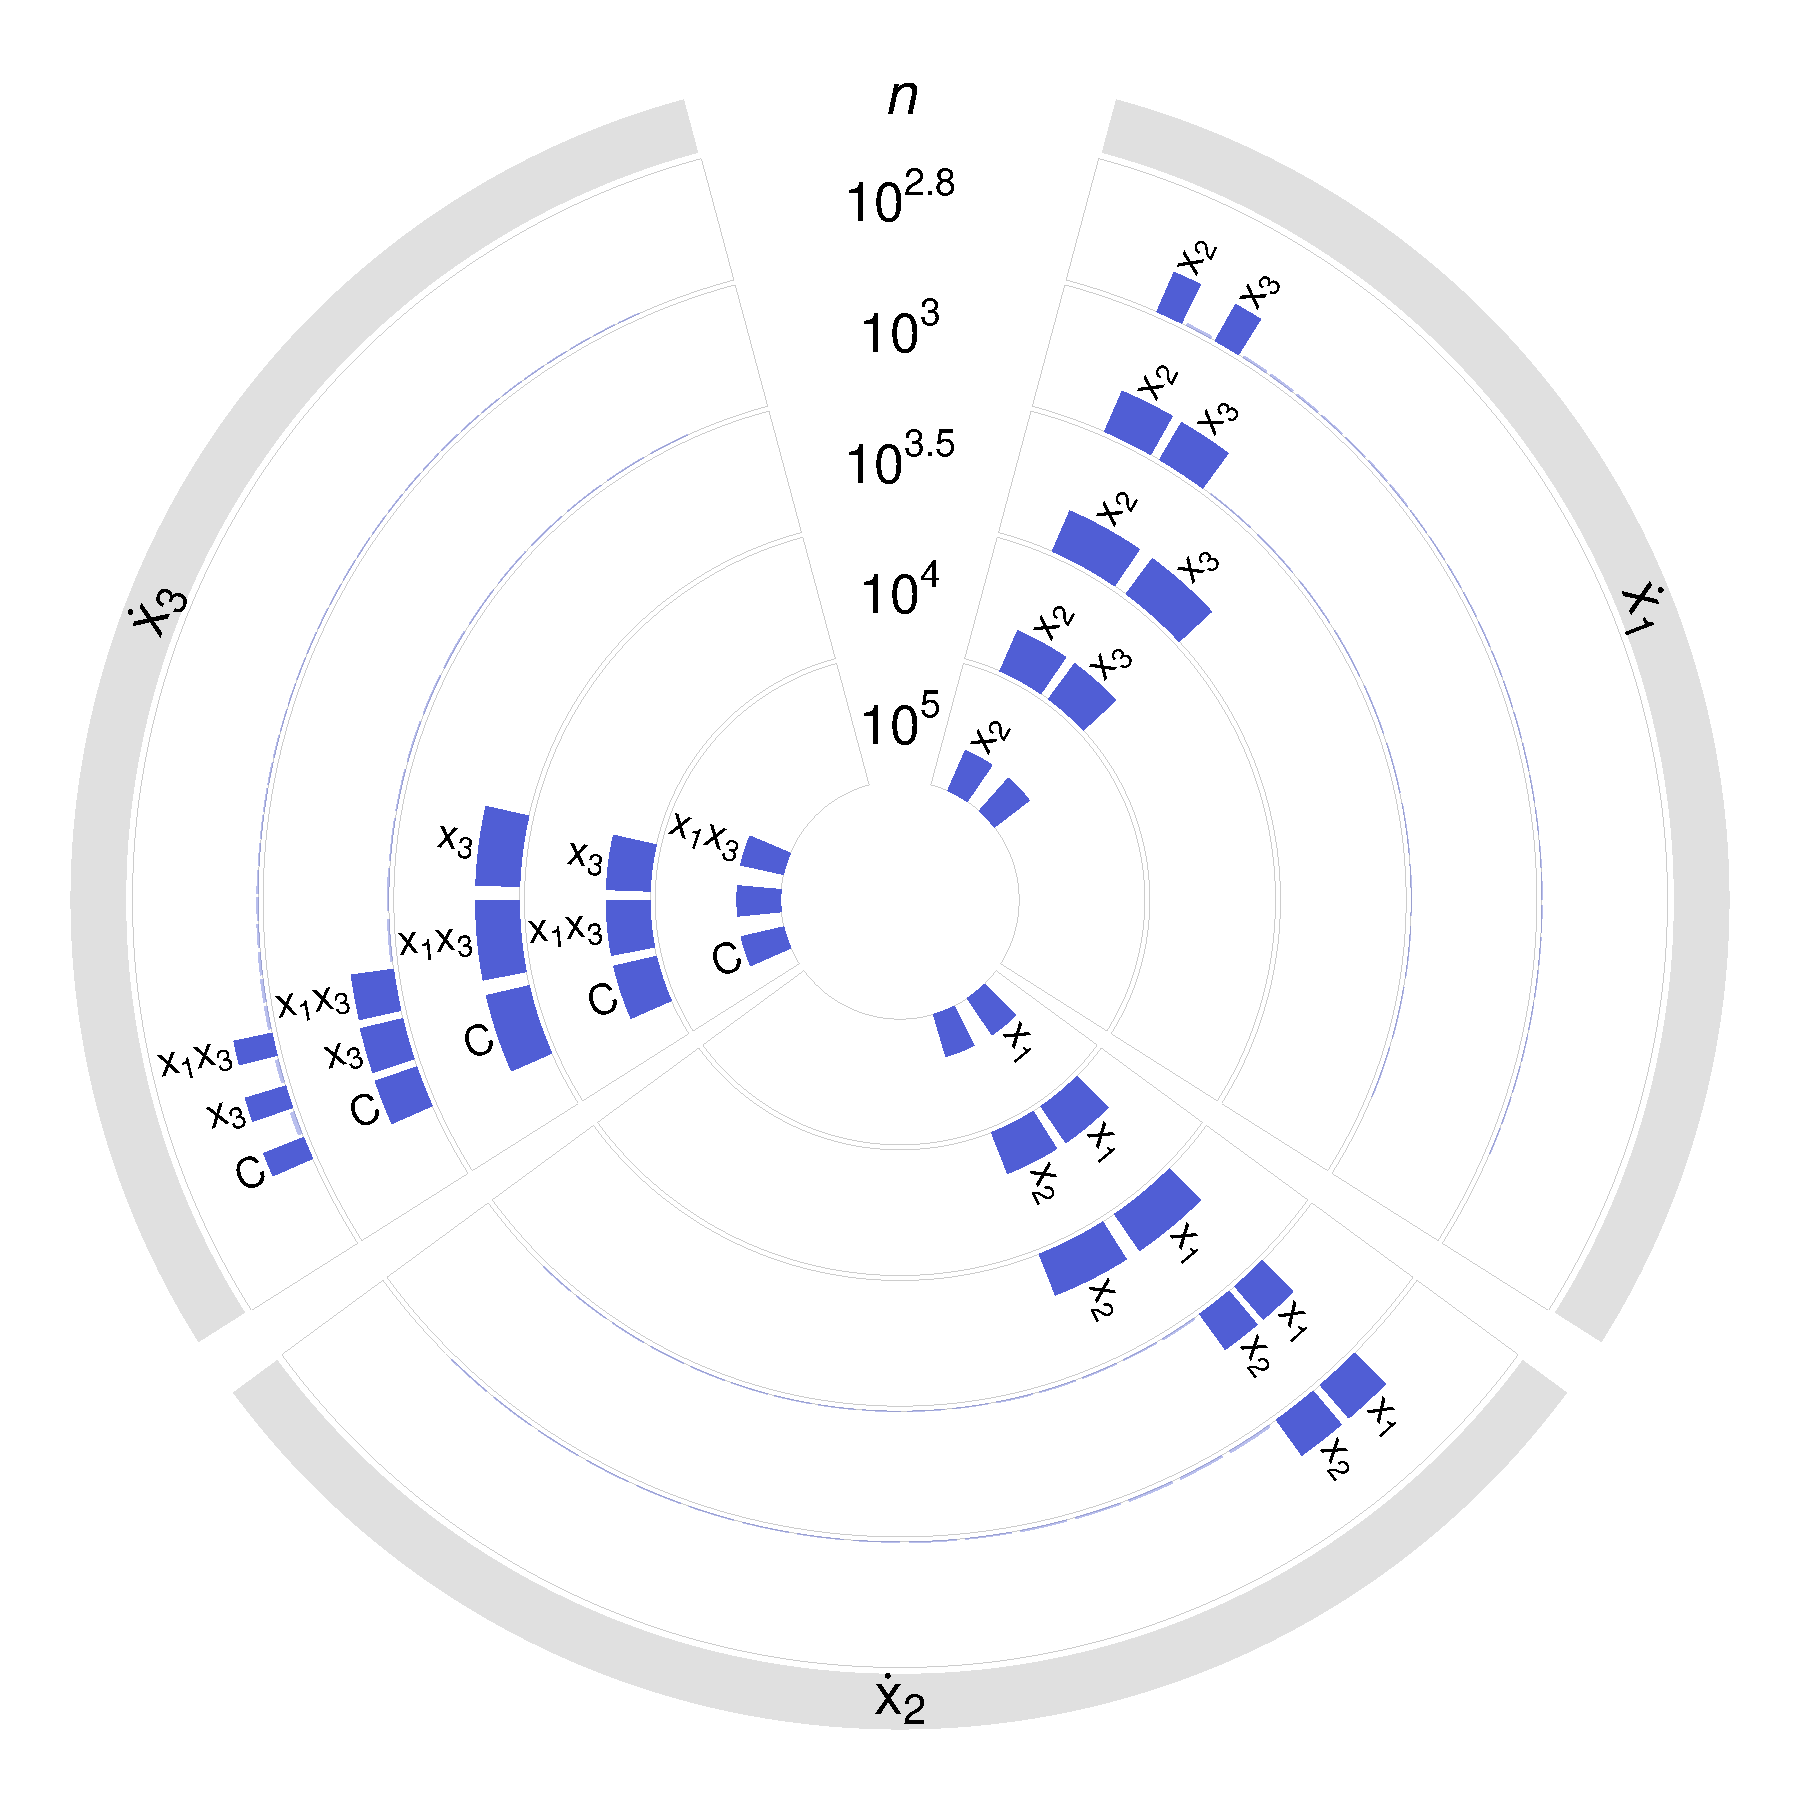
\includegraphics[width=76.000mm]{circ_rossler_n_ba.pdf}};
\node[anchor=north west, inner sep=0pt] at (83.500,4.000) {\Tag{b}};
\node[anchor=north west, inner sep=0pt] at (85.000,4.500) {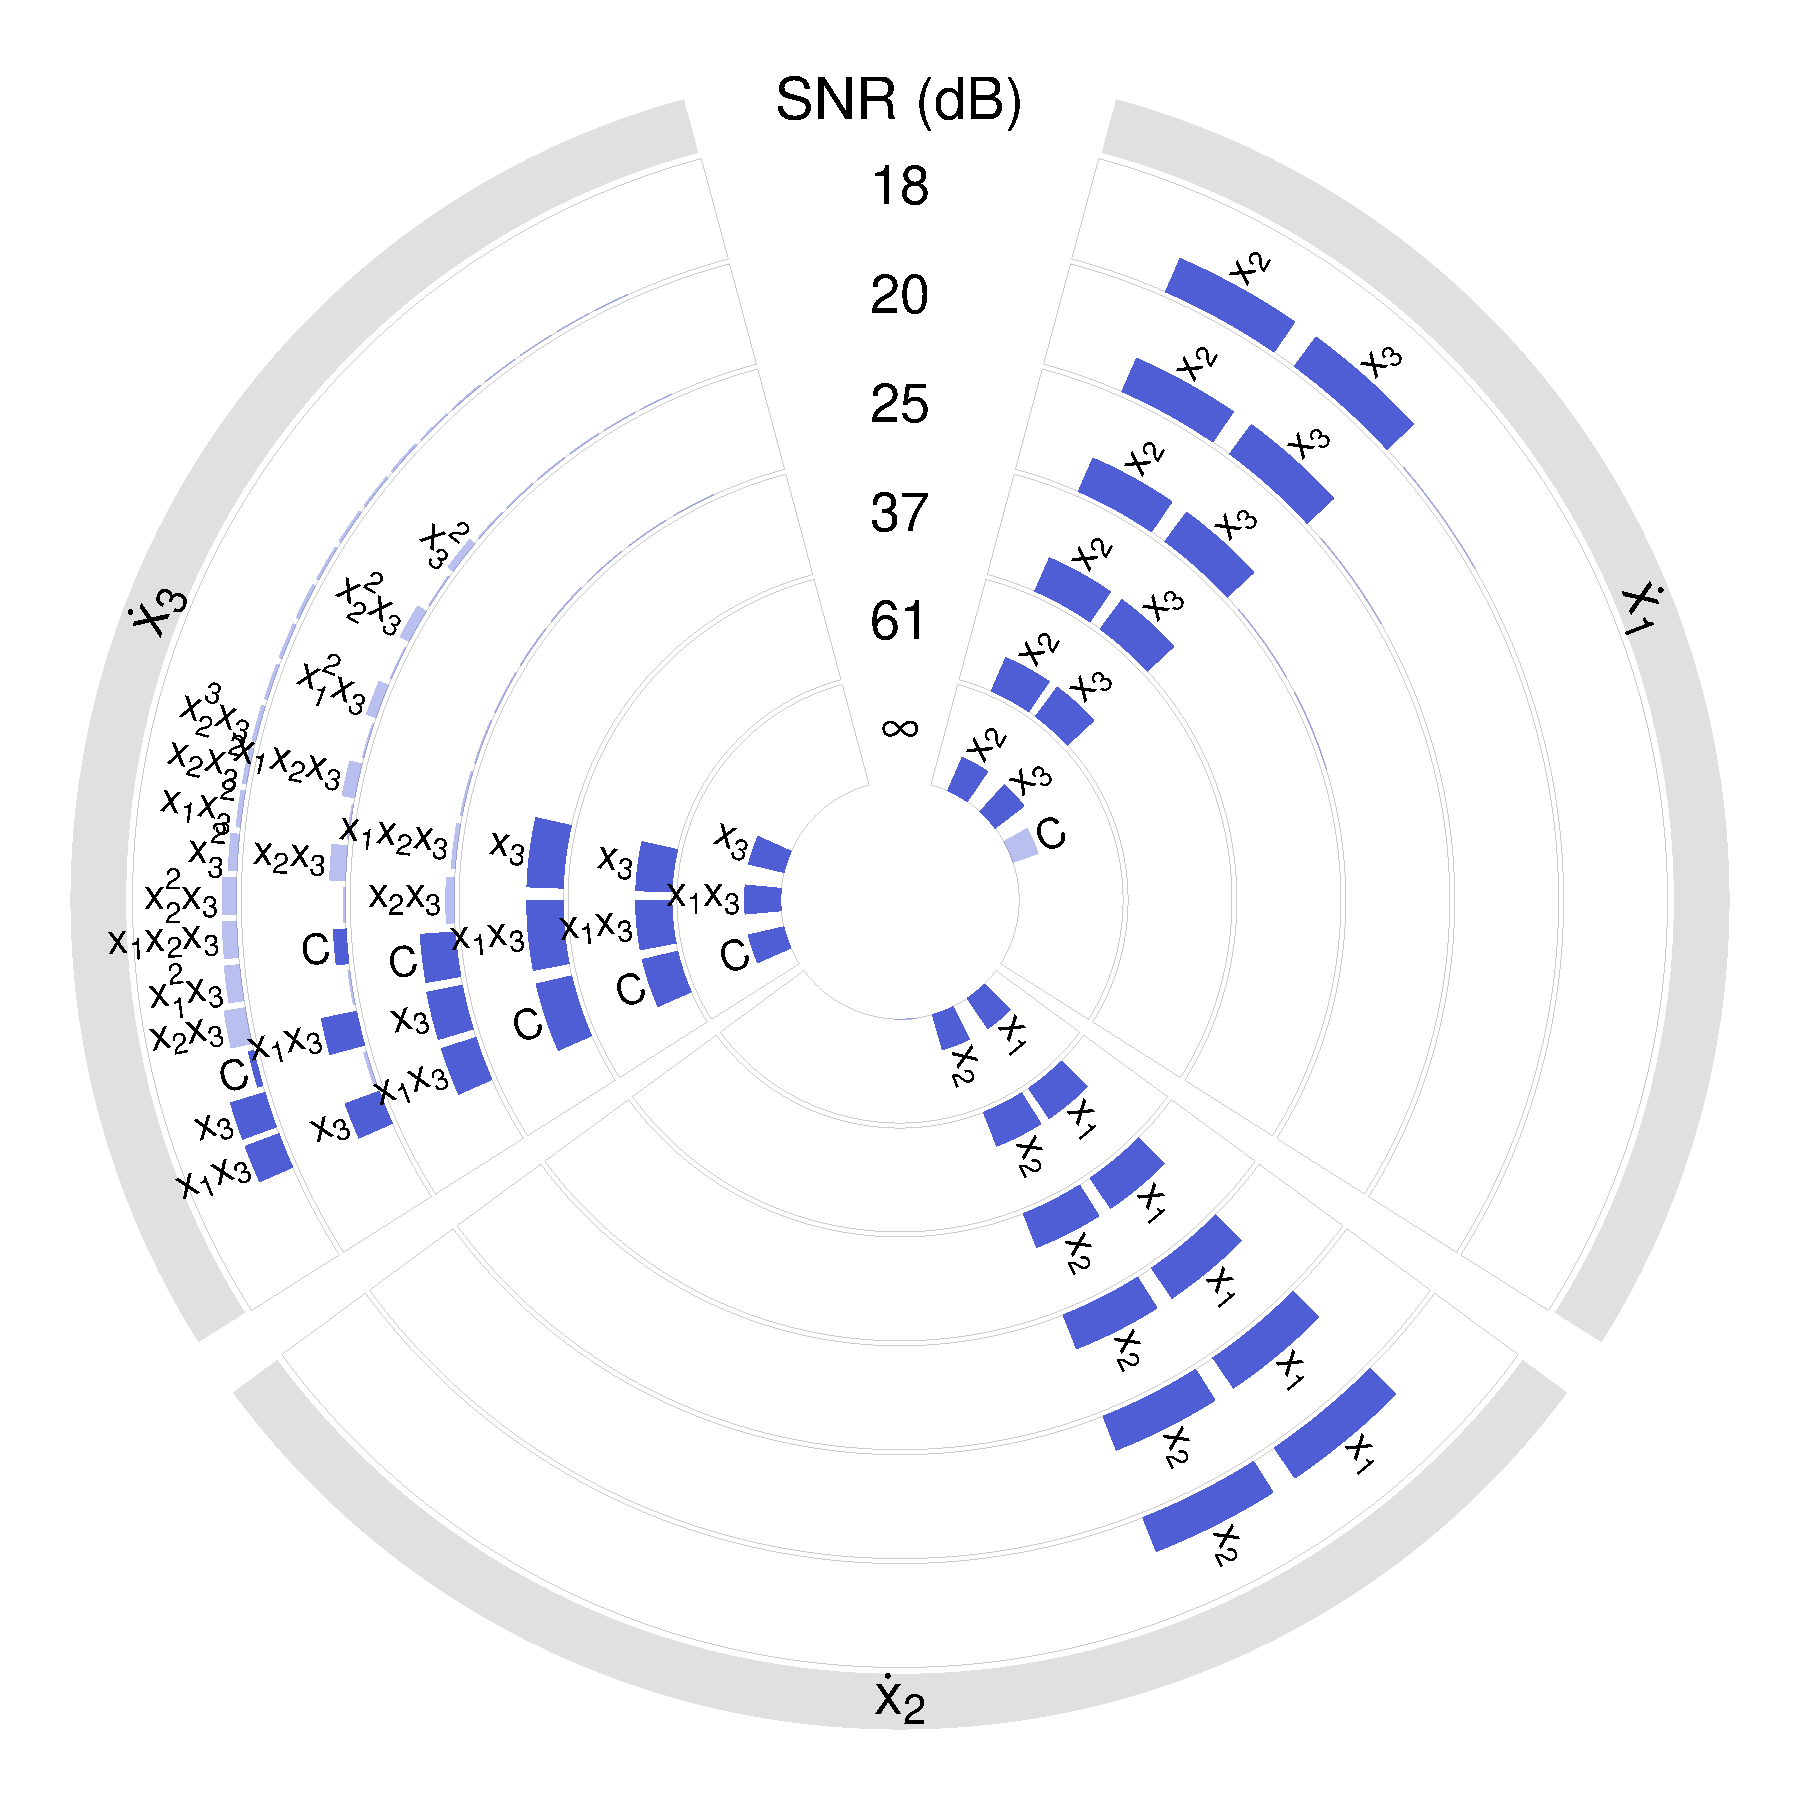
\includegraphics[width=76.000mm]{circ_rossler_snr_ba.pdf}};
\node[anchor=center, inner sep=0pt, rotate=90] at (2.000,121.500) {\Lab{ARGOS}};
\node[anchor=north west, inner sep=0pt] at (3.500,83.000) {\Tag{c}};
\node[anchor=north west, inner sep=0pt] at (5.000,83.500) {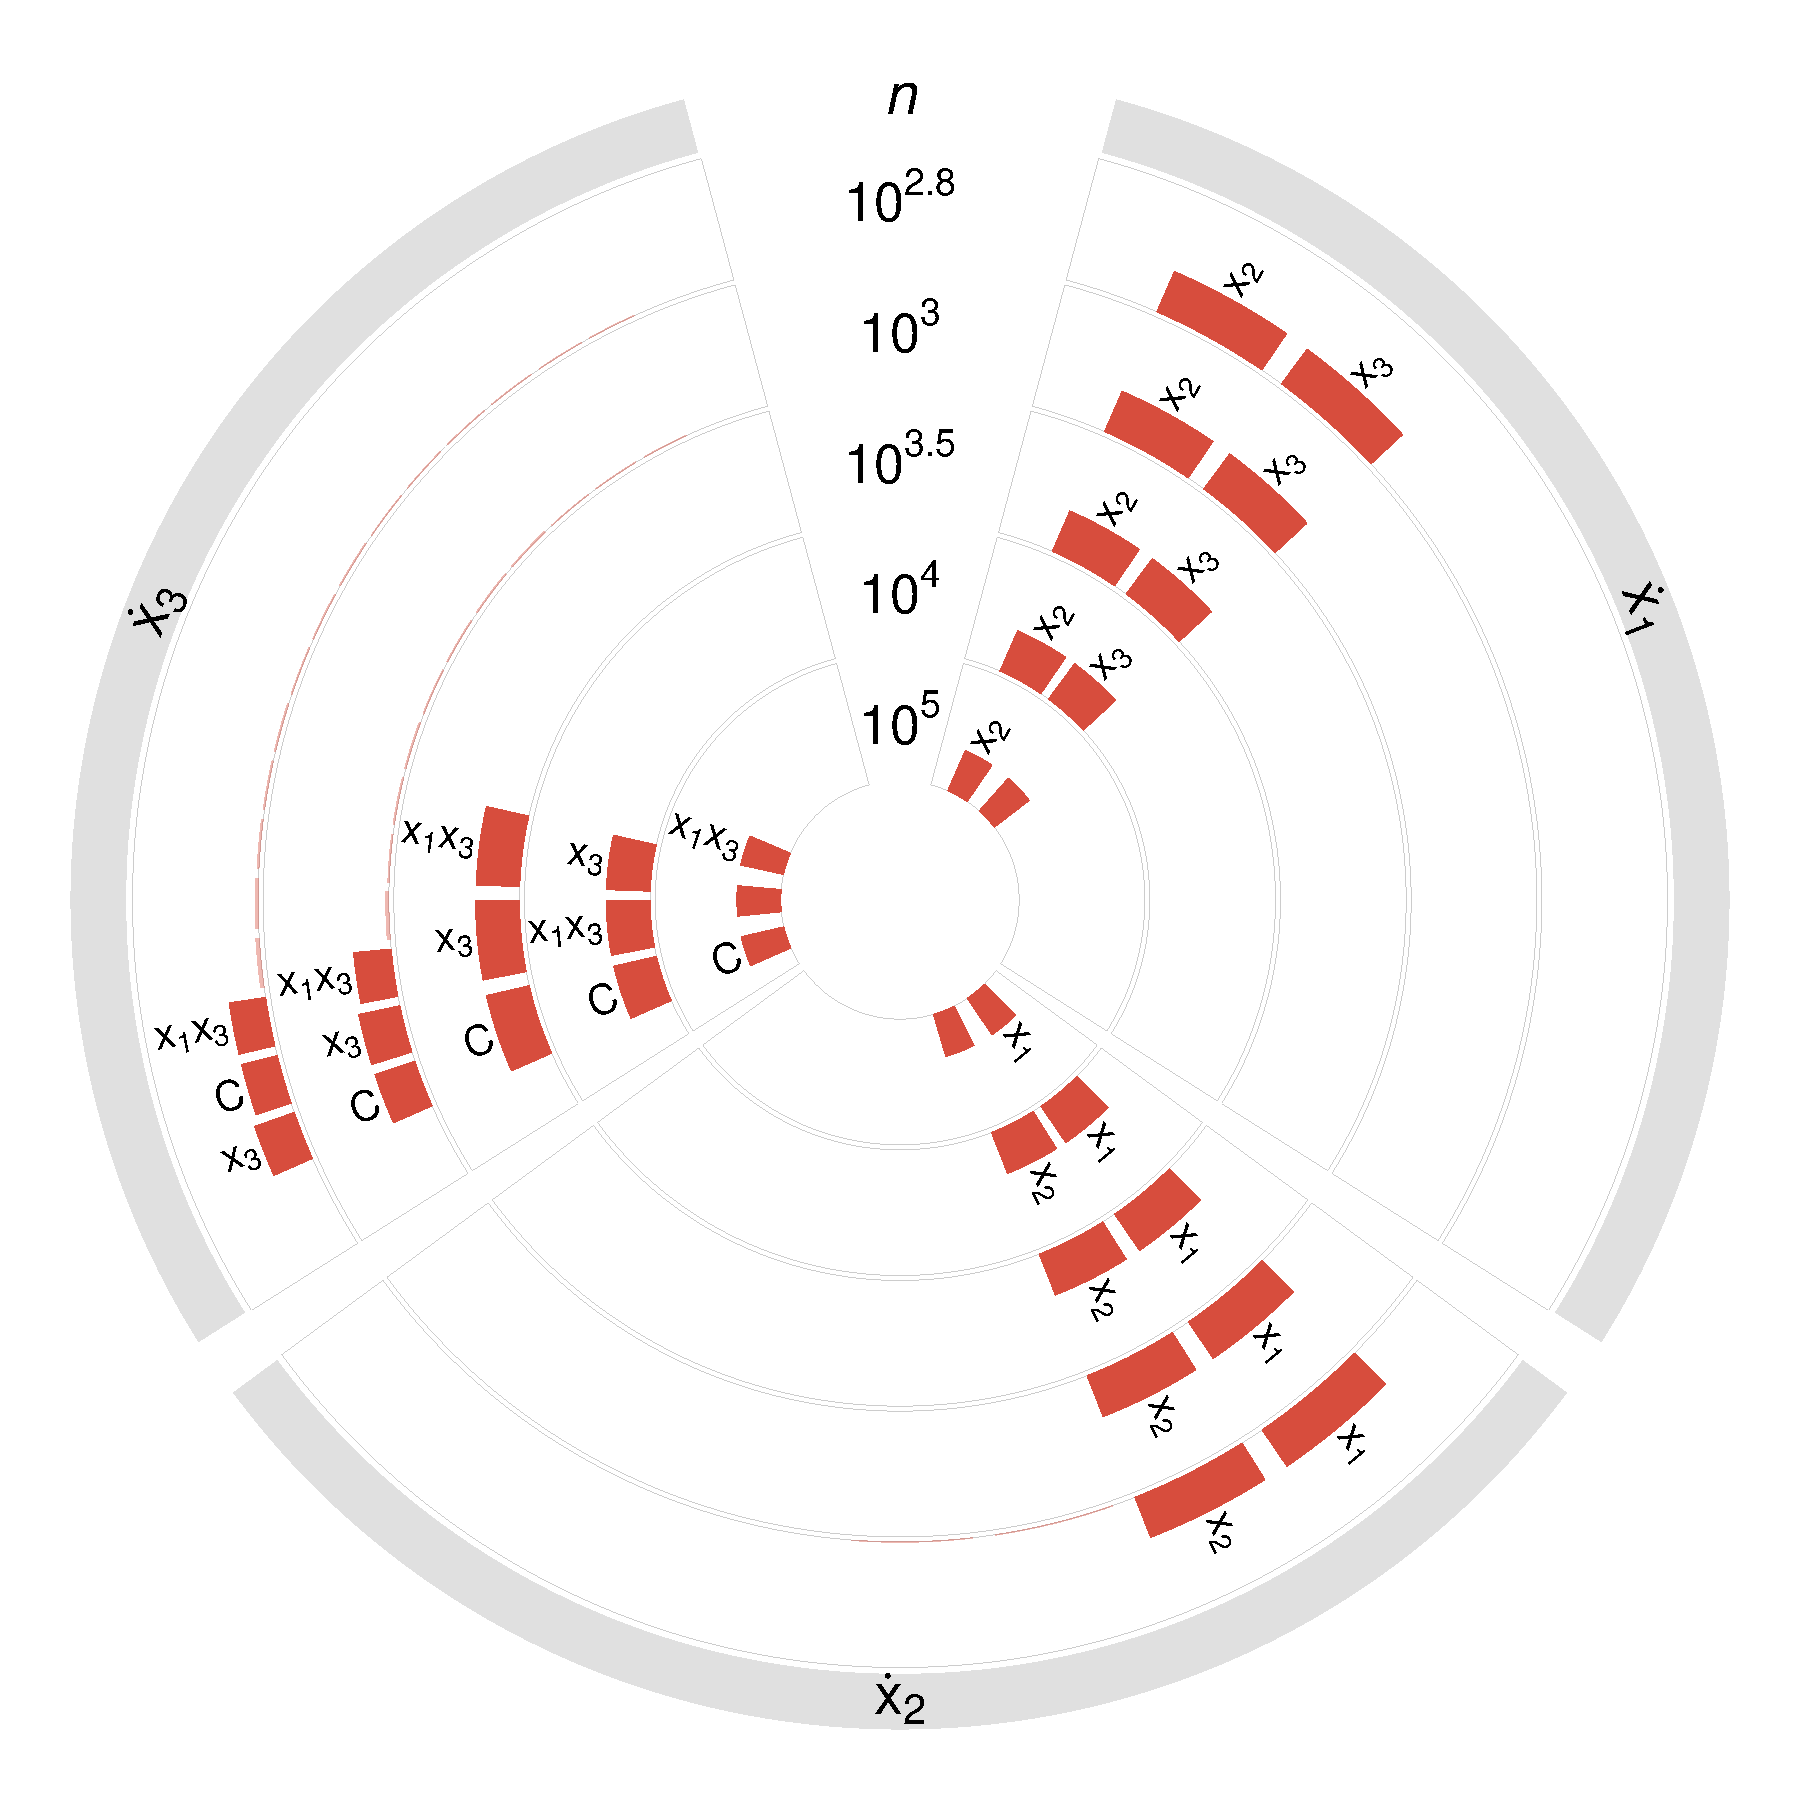
\includegraphics[width=76.000mm]{circ_rossler_n_argos.pdf}};
\node[anchor=north west, inner sep=0pt] at (83.500,83.000) {\Tag{d}};
\node[anchor=north west, inner sep=0pt] at (85.000,83.500) {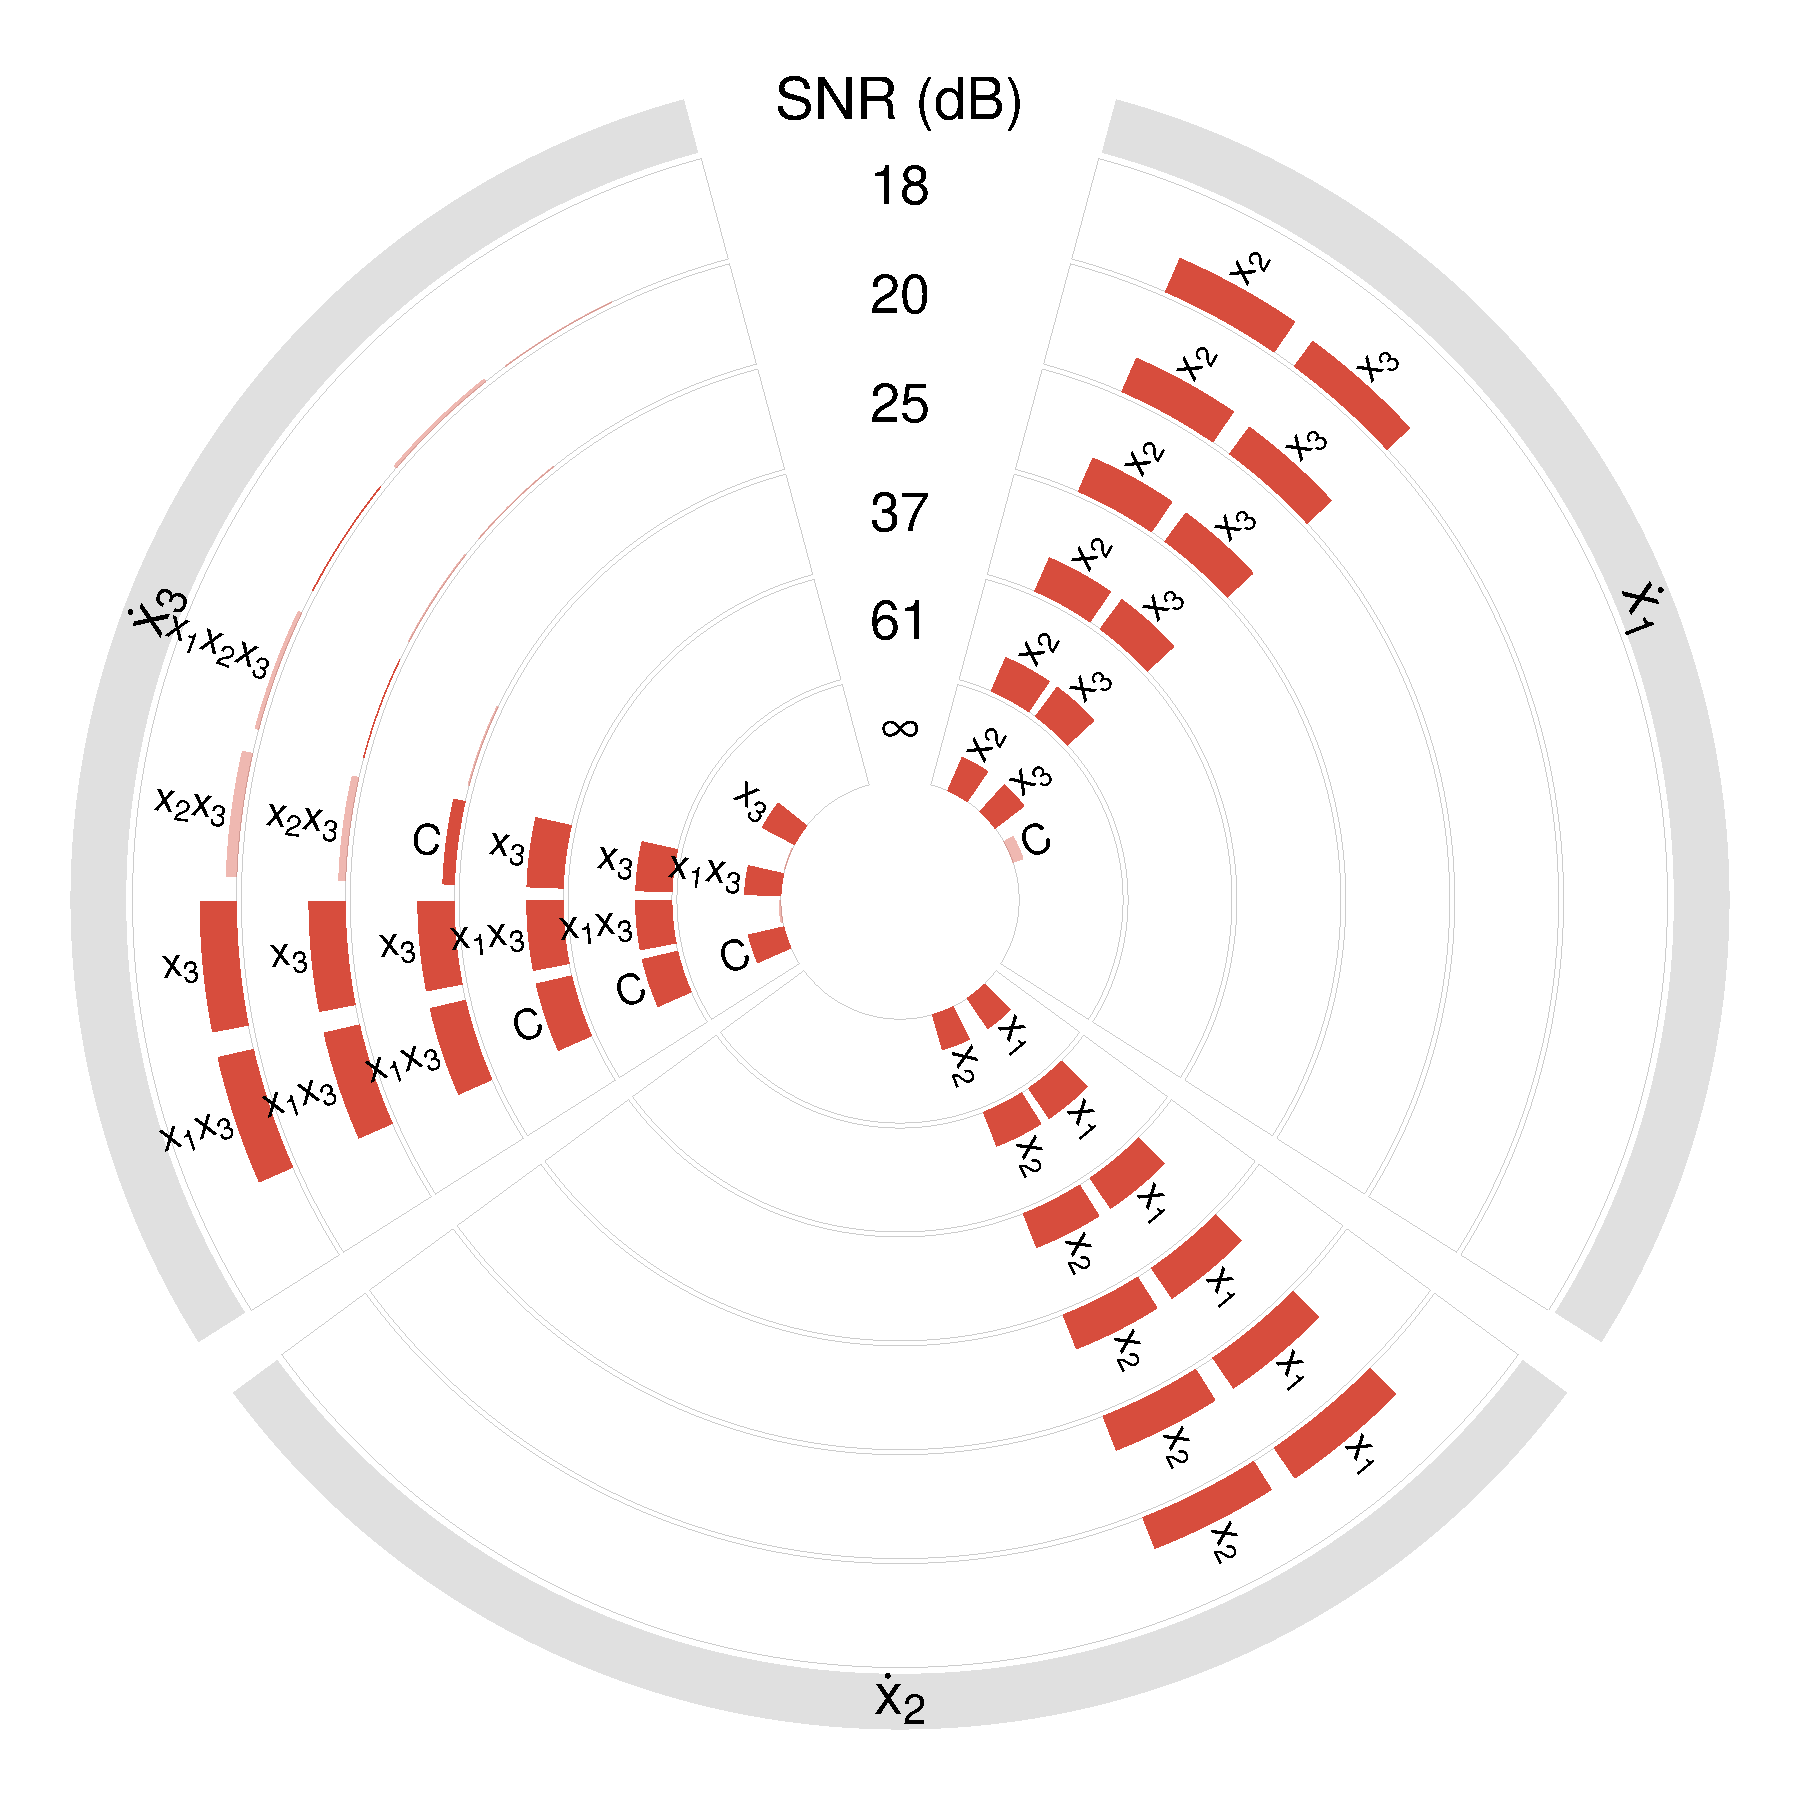
\includegraphics[width=76.000mm]{circ_rossler_snr_argos.pdf}};
\node[anchor=center, inner sep=0pt, rotate=90] at (2.000,200.500) {\Lab{SINDy}};
\node[anchor=north west, inner sep=0pt] at (3.500,162.000) {\Tag{e}};
\node[anchor=north west, inner sep=0pt] at (5.000,162.500) {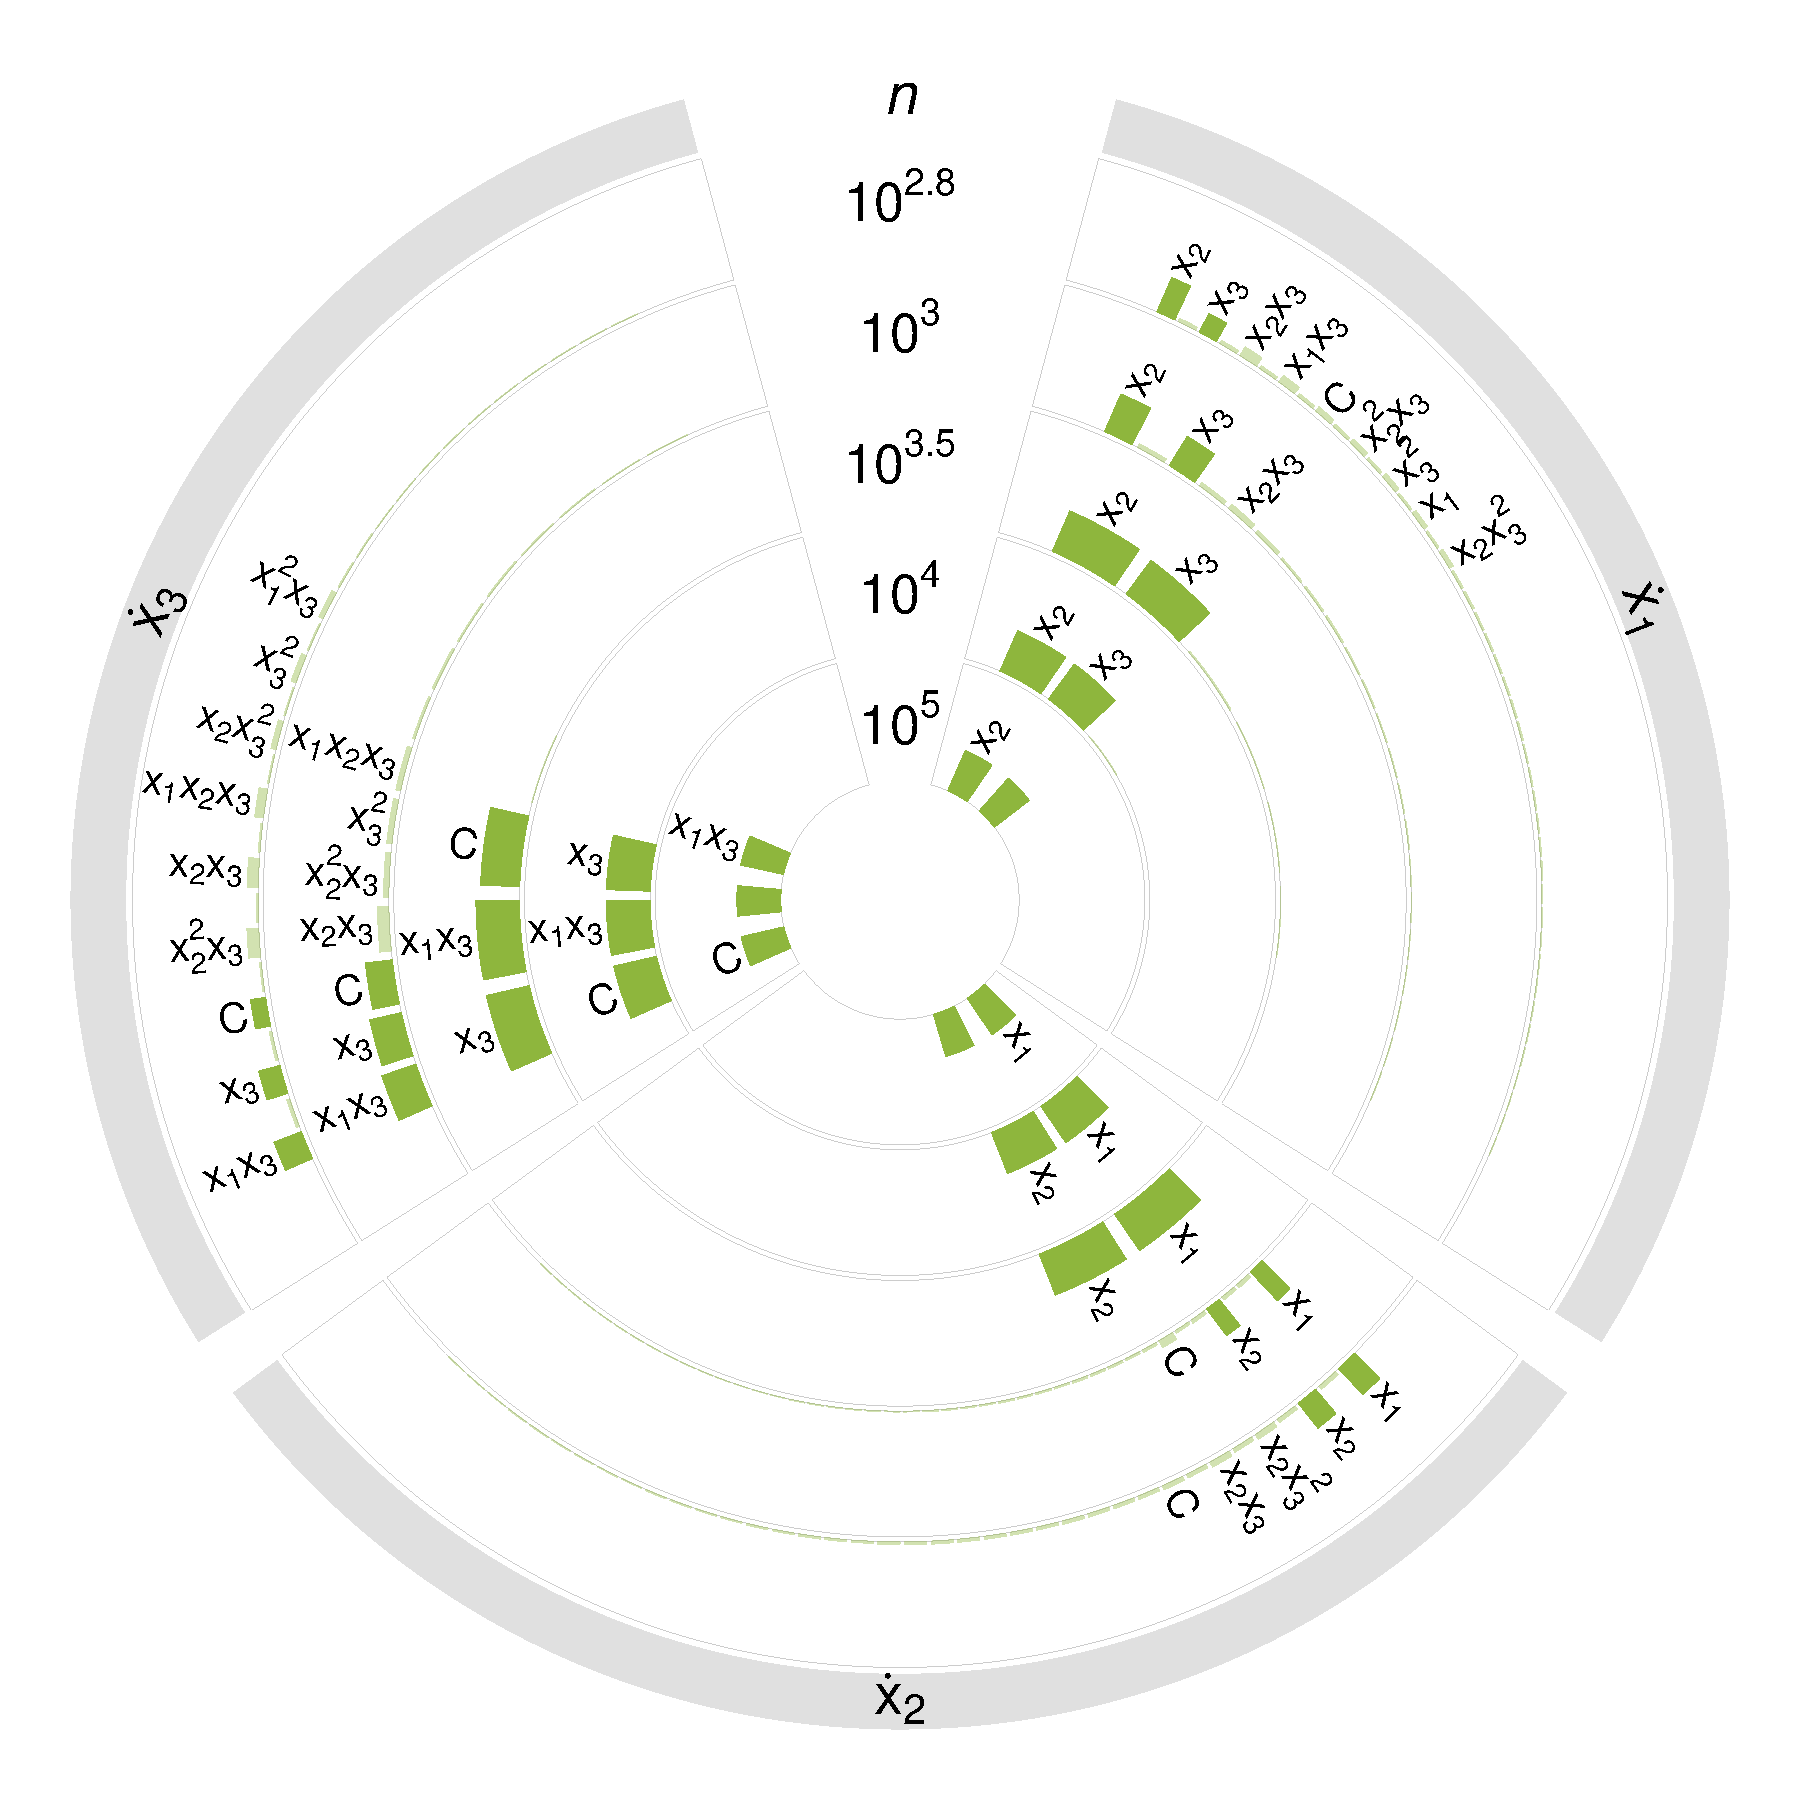
\includegraphics[width=76.000mm]{circ_rossler_n_sindy.pdf}};
\node[anchor=north west, inner sep=0pt] at (83.500,162.000) {\Tag{f}};
\node[anchor=north west, inner sep=0pt] at (85.000,162.500) {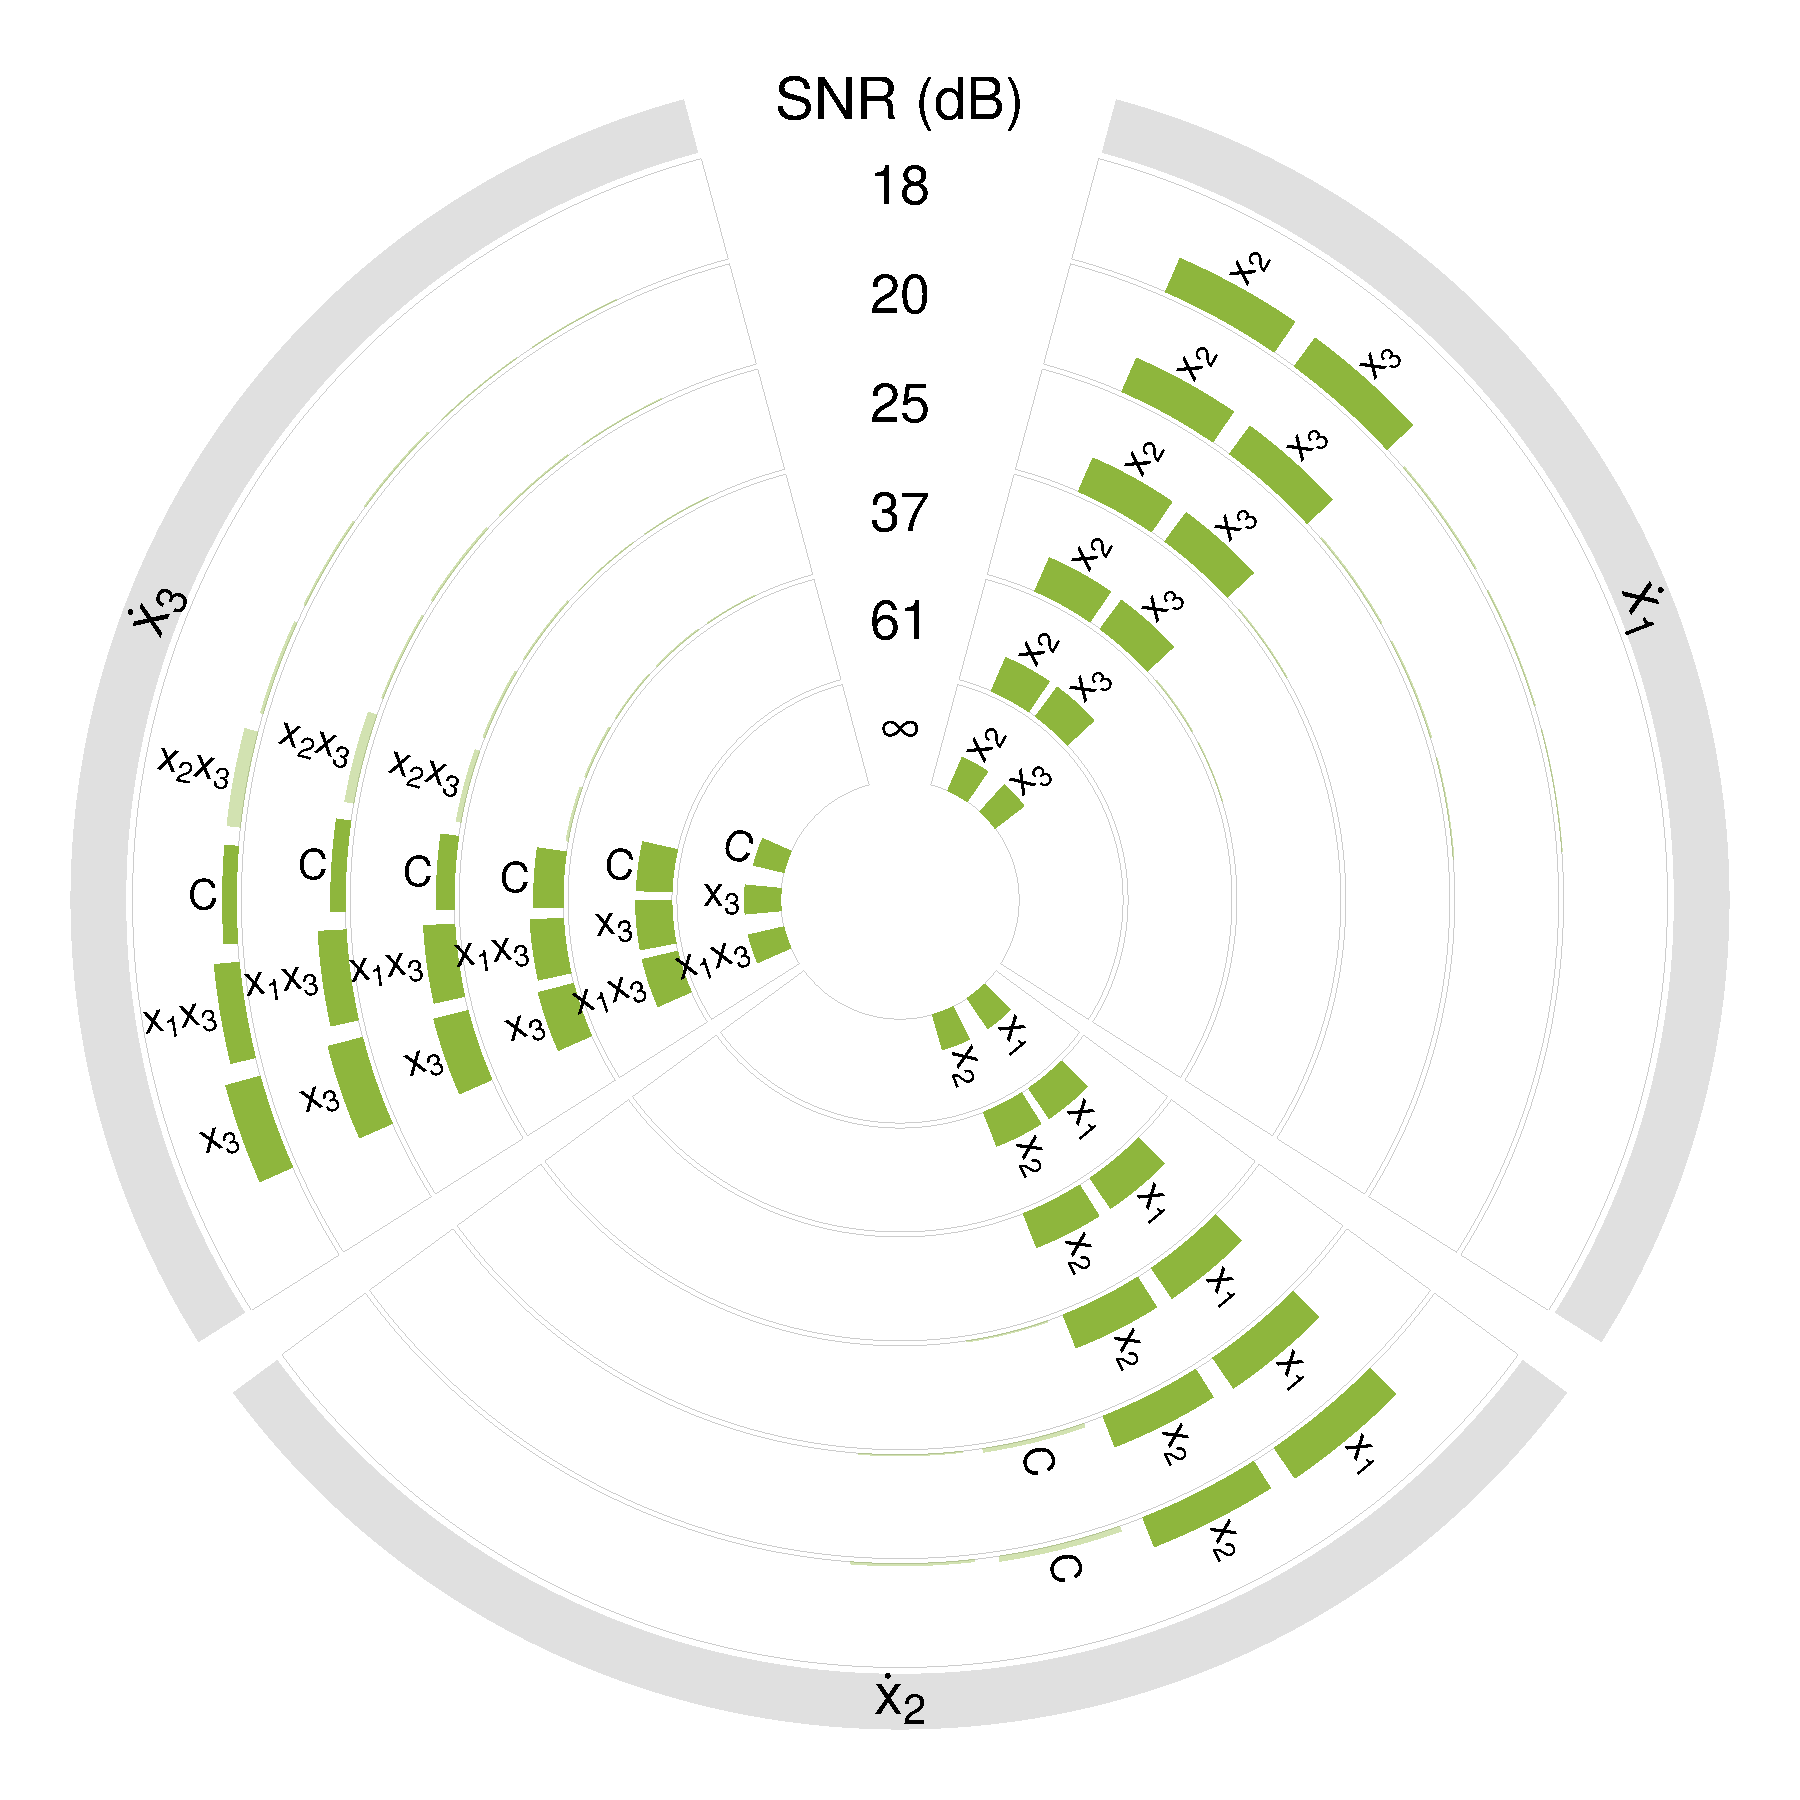
\includegraphics[width=76.000mm]{circ_rossler_snr_sindy.pdf}};
\fill[ba] (22.500,240.000) rectangle ++(2.000,2.000);
\fill[argos] (24.900,240.000) rectangle ++(2.000,2.000);
\fill[sindy] (27.300,240.000) rectangle ++(2.000,2.000);
\node[anchor=west, inner sep=0pt] at (30.500,241.000) {\Lab{true terms}};
\fill[ba!40] (44.500,240.000) rectangle ++(2.000,2.000);
\fill[argos!40] (46.900,240.000) rectangle ++(2.000,2.000);
\fill[sindy!40] (49.300,240.000) rectangle ++(2.000,2.000);
\node[anchor=west, inner sep=0pt] at (52.500,241.000) {\Lab{spurious terms}};
\node[anchor=west, inner sep=0pt] at (73.500,241.000) {\Lab{bar height: selection frequency over 100 trials}};
\end{tikzpicture}
\end{document}
